\subsection{SE-04 Consultar periodos de ETS asignados al docente}

\begin{figure}[htbp!]
	\begin{center}
		\fbox{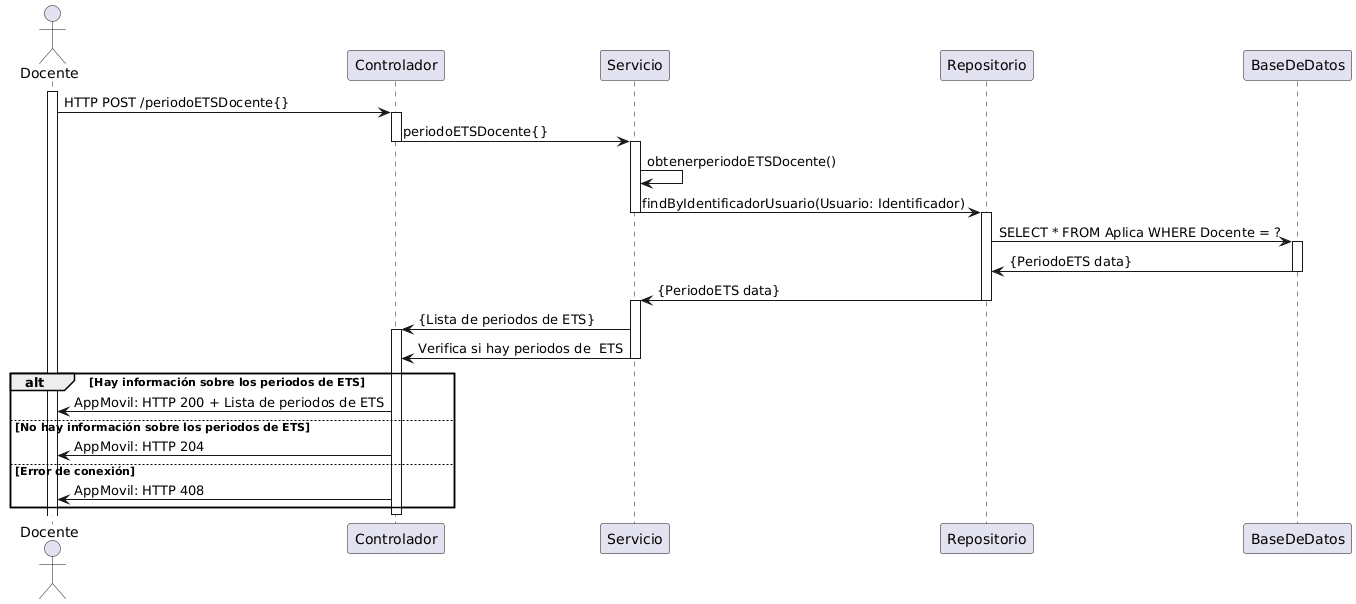
\includegraphics[width=1\textwidth]{Secuencia/CU-04.png}}
		\caption{Diagrama de secuencia del caso de uso número 04 (Consultar periodos de ETS asignados al docente).}
		\label{fig:Diagrama de secuencia CU-04}
	\end{center}
\end{figure}

En el diagrama de secuencia \ref{fig:Diagrama de secuencia CU-04} se describe el proceso planeado para el caso de uso \hyperlink{CU-04}{CU-04 Consultar periodos de ETS asignados al docente}, mostrando las interacciones que tendrá con la vista, el controlador, el servicio, el repositorio y la base de datos.

\newpage